%\begin{frame}
%\frametitle{Implementazione}
%Per la definizione della struttura, si è preso spunto da \textbf{icmp tunnel}. 
%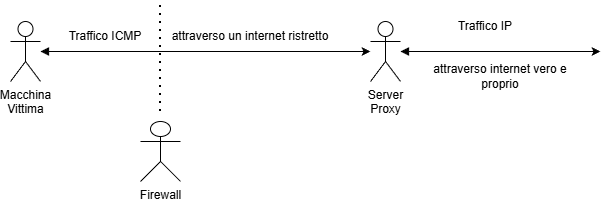
\includegraphics[width=0.7\textwidth]{../Tesi/img/ICMPtunnel/architettura_generale.png} 
%\captionof{figure}{Architettura generale di \textbf{icmp tunnel}} 
%\end{frame}
%\begin{frame}
%La struttura della comunicazione fra la macchina vittima e il proxy è la 
%seguente. \newline
%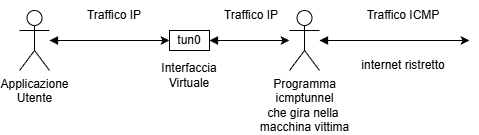
\includegraphics[width=0.65\textwidth]{../Tesi/img/ICMPtunnel/architettura_vittima.png} 
%\captionof{figure}{Comunicazione vitttima-proxy in \textbf{icmp tunnel}} 
%\textit{Icmp tunnel} che è in esecuzione sulla macchina vititma, 
%Si reindirizza il traffico IP ad un interfaccia virtuale per poi reinoltrarlo 
%al proxy tramite il protocollo ICMP.
%\end{frame}
%\begin{frame} 
%Intanto il proxy rimane in ascolto di questi pacchetti ICMP e poi li invia, 
%utilizzando il protocollo IP, verso la destinazione finale. 
%Successivamente i pacchetti in entrata nel proxy, che contengono le 
%informazioni da inoltrate alla macchina vittima, vengono incapsulati tramite 
%il protocollo ICMP ed inoltrati alla vittima. \newline
%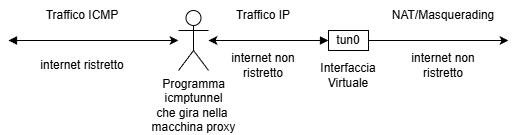
\includegraphics[width=0.65\textwidth]{../Tesi/img/ICMPtunnel/architettura_proxy.png} 
%\captionof{figure}{Comunicazione proxy-internet in \textbf{icmp tunnel}}     
%\end{frame}

\begin{frame}
\frametitle{Struttura dela comunicazione}
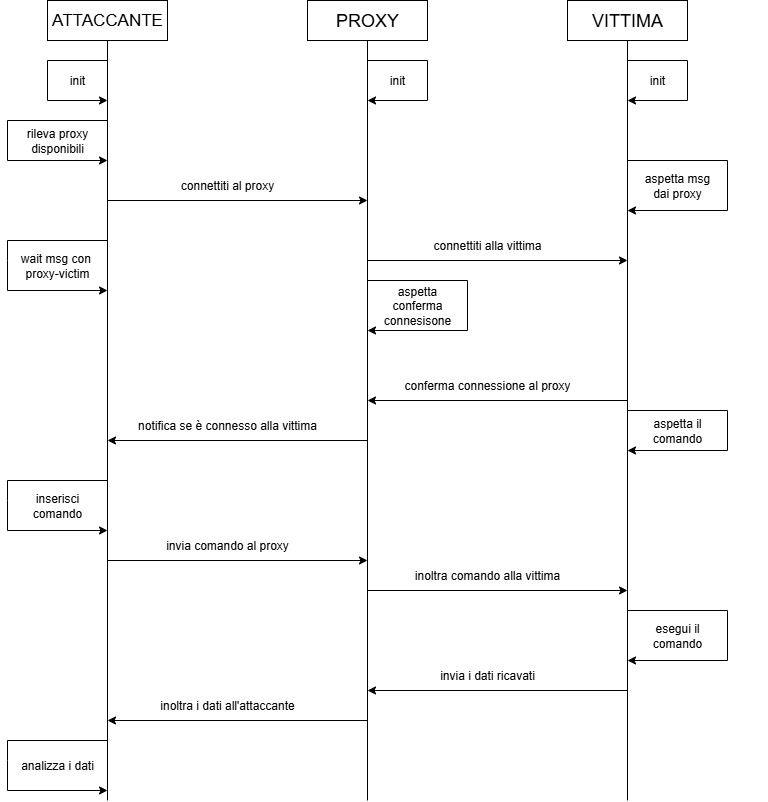
\includegraphics[width=0.6\textwidth]{../Tesi/img/implementazione/diagramma_struttura_entita.jpg} 
\captionof{figure}{Flusso di comunicazione fra le entita}
\end{frame} 

\begin{frame}
\frametitle{Struttura dell'attaccante} 
\scriptsize 
\begin{longtable}{|p{0.15\textwidth}|p{0.8\textwidth}|} 
    \hline 
    \textbf{Opzione} & \textbf{Utilizzo}  \\
    \hline
    Path file & 
    Percorso per il file di configuraizone da caricare. In questo file JSON viene specificato 
    l'indirizzo IP della vittima, la metodologia di attacco e la lista dei proxy che si vogliono usare. 
    \\ \hline 
    %\caption{Opzioni richieste nel comando dell'attaccante} 
\end{longtable} 
\normalsize
%Tramite la linea di comando, che ha lanciato lo script, 
%si ricava il valore del percorso per il file di  
Tramite il file di configurazione specificato, l'attaccante definisce
%configurazione dell'attacccante. In esso viene definito 
l'\textbf{indirizzo IP della vittima}, il 
\textbf{metodo di attacco} per l'esfiltrazione dei dati ed 
i \textbf{proxy che si vogliono utilizzare} 
verificando successivamente quali (fra quelli 
specificati) sono utiizzabili. 
\vspace{1ex} \newline
Dopodichè inserirà il 
comando che si vorrà far eseguire dalla vititma (o 
i dati che gli si vuole mandare).  
Una volta ricevuti tutti i pacchetti, %dai proxy, 
li riordinerà per ricavare correttamente il dato  
esfiltrato ed infine potrà decidere se invire un 
ulteriore comando o se terminare la comunicazione. 
%In quest'ultimo caso, notificherà l'evento a ciascuno 
%dei proxy. 
\end{frame}  
%\begin{frame} 
%\begin{columns}[T,onlytextwidth]
%\column{0.48\textwidth}   
%\justifying 
%%Nel caso non si abia una connessione diretta con la 
%%vittima ma si utilizzino dei proxy come intermediari, 
%%si aspetterà che essi inoltrino i dati che la vittima 
%%ha inviato a ciascuno di essi. 
%Una volta ricevuti tutti i pacchetti, %dai proxy, 
%l'attaccante li riordinerà per ricavare il messaggio 
%correttamente. Infine potrà decidere se invire un 
%ulteriore comando o se terminare la comunicazione. 
%%In quest'ultimo caso, notificherà l'evento a ciascuno 
%%dei proxy. 
%\column{0.48\textwidth} 
%%\begin{figure}
%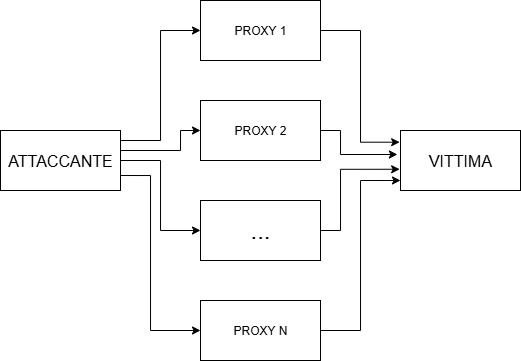
\includegraphics[width=\textwidth]{../Tesi/img/implementazione/struttura attacker.proxy.victim 3.jpg} 
%%\captionof{figure}{Struttura e dialogo delle entità presenti} 
%%\end{figure} 
%\end{columns}  
%\end{frame} 

\begin{frame} 
\frametitle{Struttura del Proxy} 
\scriptsize 
\begin{longtable}{|p{0.2\textwidth}|p{0.75\textwidth}|} 
    \hline 
    \textbf{Opzione} & \textbf{Utilizzo}  \\
    \hline
    Indirizzo IP & 
    Rappresenta l'indirizzo IP dell'attaccante.
    \\ \hline 
    %\caption{Opzioni richieste nel comando del proxy} 
\end{longtable} 
\normalsize 
Durante la fase di inizializzazione il proxy necessita 
di sapere l'indirizzo IP dell'attaccante così da 
stabilire una connessione solamente con lui; 
tutti i tentativi di connessione provenienti da 
indirizzi diversi verranno scartati. 
\vspace{1ex} \newline 
Una volta stabilita la connessione, il proxy aspetterà 
che l'attaccante gli invii l'indirizzo IP della 
vittima ed il metodo di attaco scelto. 
Ricevuto l'indirizzo il proxy si assicurerà che la 
comunicazione con esso sia possibile. Nel caso non 
sia possibile, il proxy aggiornerà l'attaccante che 
non potrà essere utilizzato per l'esfiltrazione dei 
dati dalla vittima. Entrambe le entità procederanno 
poi alla chiusura della comunicazione.
\end{frame} 
\begin{frame} 
I successivi messaggi da parte dell'attaccante 
potranno essere: 
\begin{itemize} 
    \item Il messaggio indicante il comando da inoltrare alla vittima. 
    \item Il messagio indicante che il proxy non ha 
    ricevuto il comando e che dovrà procedere ad 
    ascoltare i dati provenienti dalla vittima. 
    \item Il messaggio indicante la terminazione 
    della comunicazione. 
\end{itemize} 
Inoltrato il comando aspetta poi che la vittima 
inizi ad inviare i dati che dovranno essere poi 
inoltrati all'attaccante. 
\vspace{1ex} \newline 
Un volta terminato, rimarrà in ascolto di aggiornamenti da parte 
dell'attaccante, che potranno essere o un nuovo comando oppure la notifica 
sulla chiusura della comunicazione. Nel secondo caso provvederà ad aggiornare 
la vittima della cosa. 
\end{frame} 

\begin{frame} 
\frametitle{Vittima}
\frametitle{Struttura Vittima}
\scriptsize 
\begin{longtable}{|p{0.3\textwidth}|p{0.65\textwidth}|} 
    \hline 
    \textbf{Opzione} & \textbf{Utilizzo}  \\
    \hline
    Numero connesisoni & 
    Numero minimo di connesisoni necessarie per 
    l'esecuzione dell'attacco. 
    %Soddisfatto il requisito, la vittima continua con l'esecuzione del comando. 
    \\  \hline 
    %\caption{Opzioni richieste nel comando della vittima} 
\end{longtable} 
\normalsize 
Nella fase di inizializzazione alla vittima verranno 
indicate la quantità di connessioni attive necessarie 
per l'esecuzione dell'attacco. Queste connessioni 
verranno poi usate sia per la ricezione del comando 
che per l'esfiltrazione dei dati. 
\vspace{1ex} \newline 
In questa fase, il proxy (o l'attaccante) che 
si vuole connettere indicherà alla vittima anche 
l'attacco che si userà per lo scambio dei dati. 
\vspace{1ex} \newline 
Definiti i porxy disponibili, la vittima aspetterà di 
ricevere un comando. Alla sua ricezione, lo eseguirà 
ed i dati ricavati verranno inviati all'attaccante 
tramite le connessioni precedentemente stabilite. 
\end{frame}

\begin{frame}  
\frametitle{Ulteriori aspetti relativi all'implementazione}
Si ritiene fondamentale la presenza di più 
\textbf{proxy intermediari} fra l'attaccante e la 
vittima. Ciò permette di distribuire in modo 
omogeneo il carico sulla rete che verrà generato 
dall'esfiltrazione dei dati. %Se invece si usasse 
%un singolo proxy, tutto il flusso verrà indirizzato 
%verso un'unica destinazione
\vspace{1ex} \newline 
Un limite alla \textbf{quantità di dati} inviabili 
in un intervallo di tempo ed un periodo di riposo 
prima di poterne inviare degli altri. Questo per 
permettere l'invio di file di grosse dimensioni 
evitando di congestionare il canale di comunicazione. 
\vspace{1ex} \newline 
L'invio di un \textbf{messaggi di tipo Request} 
richiede la ricezione di una risposta; che 
normalmente sarà uguale al messaggio inviato. Una 
soluzione può essere l'invio di soli messaggi di 
tipo Reply oppure la disabilitazione delle risposte 
così da poterne inviare una noi stessi. 
\end{frame} 



